\documentclass{standalone}
\usepackage{tikz}
\usetikzlibrary{patterns, positioning}
\usepackage[sfdefault]{ClearSans} %% option 'sfdefault' activates Clear Sans as the default text font
\usepackage[T1]{fontenc}

\begin{document}
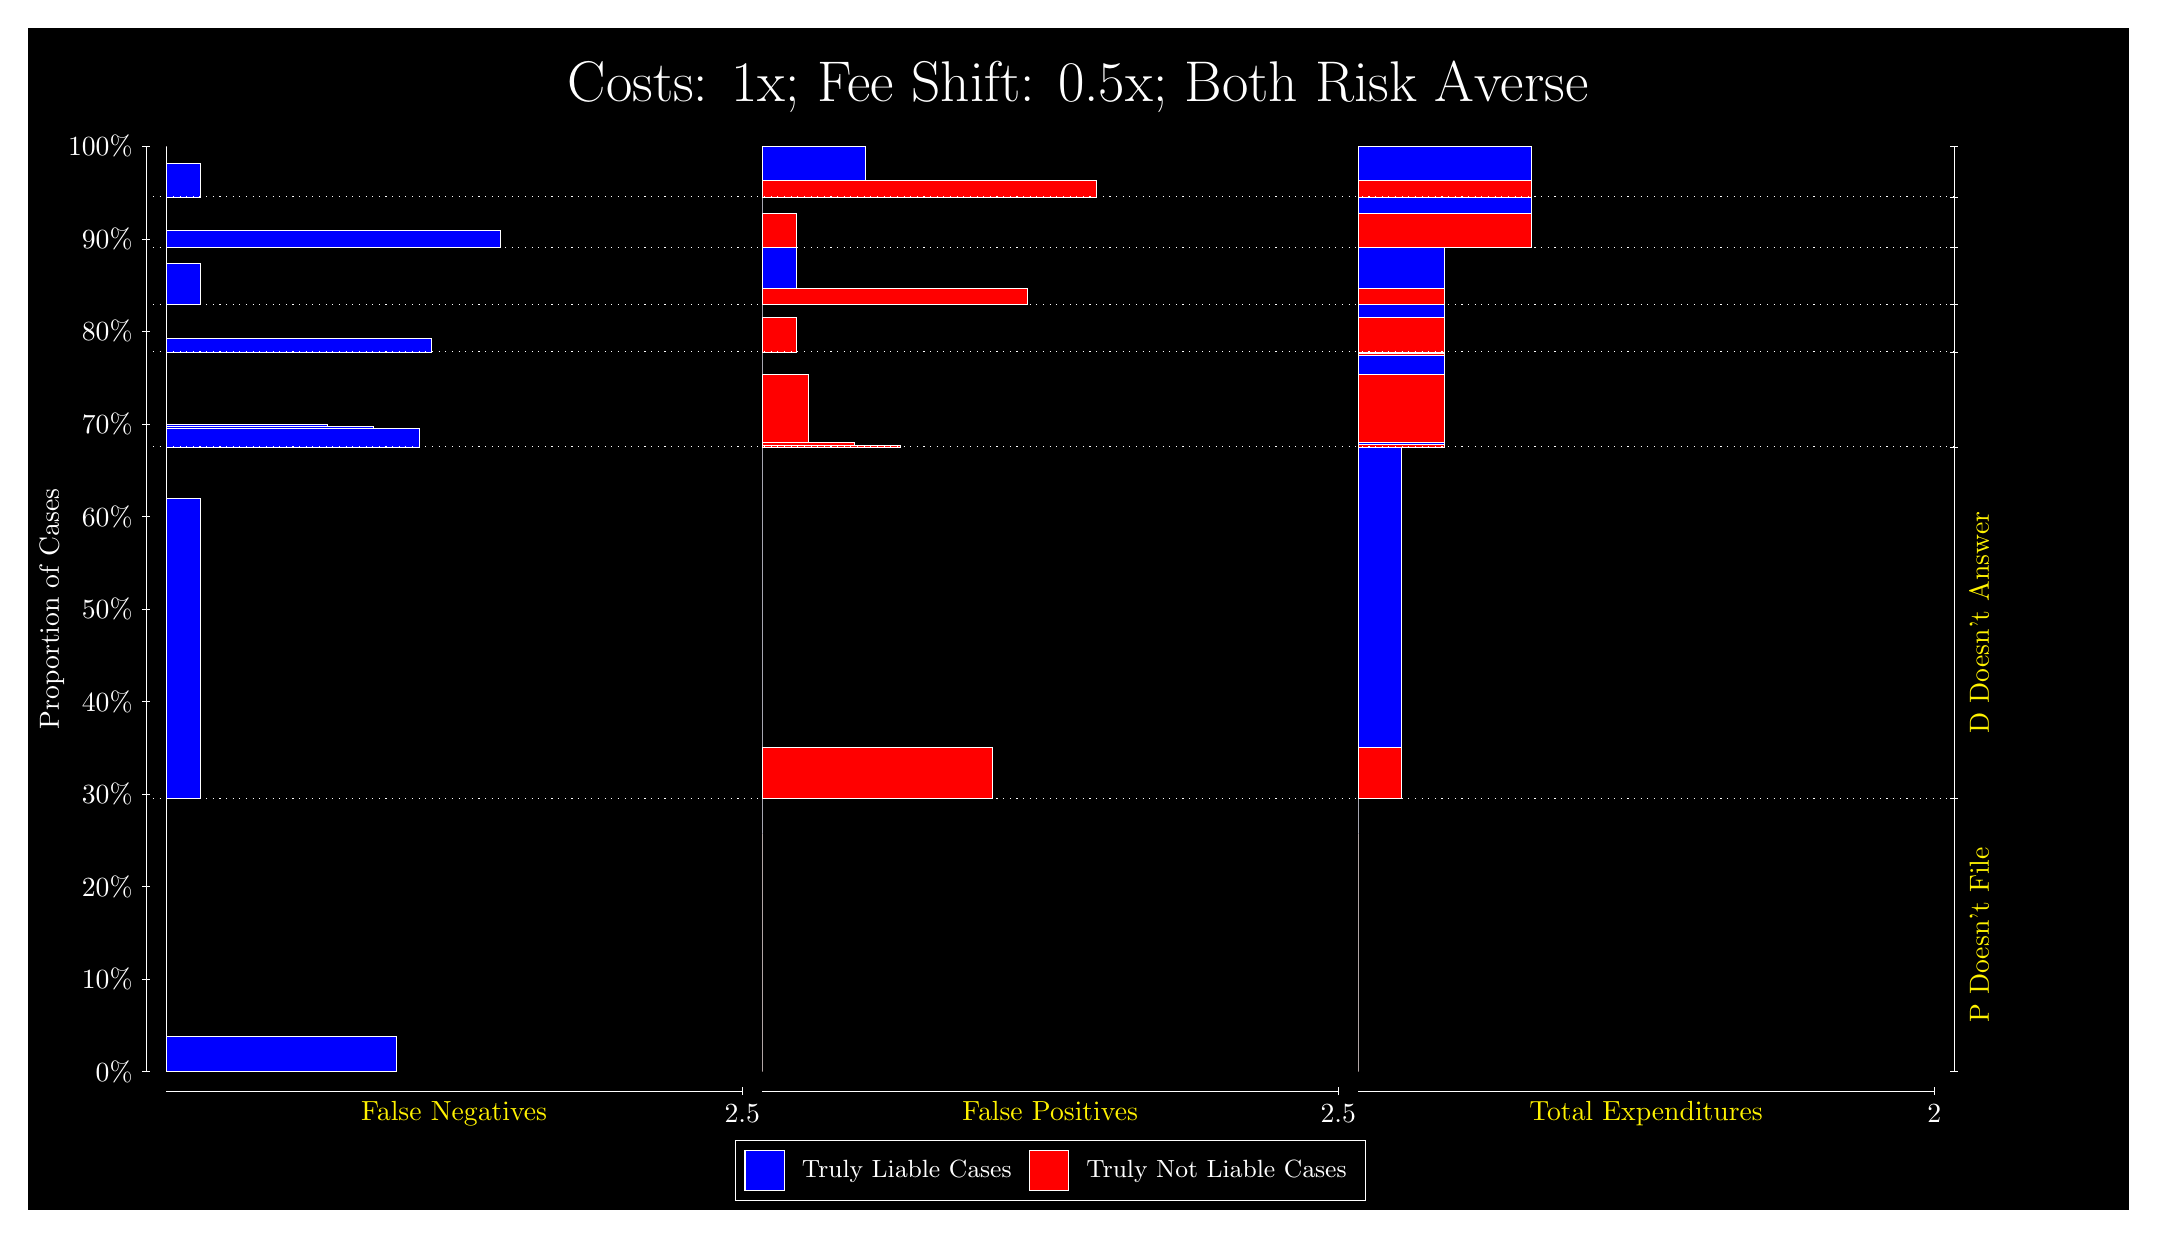
\begin{tikzpicture}
\draw[fill=black] (0,0) rectangle (26.667,15);
\draw[text=white] (0,13.5) rectangle (26.667,15) node[midway] {\huge Costs: 1x; Fee Shift: 0.5x; Both Risk Averse};
\draw[white, very thin] (1.5,1.75) -- (1.5,13.5);
\node[rotate=90, text=white, anchor=center] at (0.3, 7.625) {Proportion of Cases};
\draw[white, very thin] (1.45,1.75) -- (1.55,1.75);
\node[text=white, anchor=east] at (1.45, 1.75) {0\%};
\draw[white, very thin] (1.45,2.925) -- (1.55,2.925);
\node[text=white, anchor=east] at (1.45, 2.925) {10\%};
\draw[white, very thin] (1.45,4.1) -- (1.55,4.1);
\node[text=white, anchor=east] at (1.45, 4.1) {20\%};
\draw[white, very thin] (1.45,5.275) -- (1.55,5.275);
\node[text=white, anchor=east] at (1.45, 5.275) {30\%};
\draw[white, very thin] (1.45,6.45) -- (1.55,6.45);
\node[text=white, anchor=east] at (1.45, 6.45) {40\%};
\draw[white, very thin] (1.45,7.625) -- (1.55,7.625);
\node[text=white, anchor=east] at (1.45, 7.625) {50\%};
\draw[white, very thin] (1.45,8.8) -- (1.55,8.8);
\node[text=white, anchor=east] at (1.45, 8.8) {60\%};
\draw[white, very thin] (1.45,9.975) -- (1.55,9.975);
\node[text=white, anchor=east] at (1.45, 9.975) {70\%};
\draw[white, very thin] (1.45,11.15) -- (1.55,11.15);
\node[text=white, anchor=east] at (1.45, 11.15) {80\%};
\draw[white, very thin] (1.45,12.325) -- (1.55,12.325);
\node[text=white, anchor=east] at (1.45, 12.325) {90\%};
\draw[white, very thin] (1.45,13.5) -- (1.55,13.5);
\node[text=white, anchor=east] at (1.45, 13.5) {100\%};

\draw[white, very thin] (24.457,1.75) -- (24.457,13.5);
\draw[white, very thin] (24.407,1.75) -- (24.507,1.75);
\node[anchor=west] at (24.407, 1.75) {};
\draw[white, very thin] (24.407,5.2168) -- (24.507,5.2168);
\node[anchor=west] at (24.407, 5.2168) {};
\draw[white, very thin] (24.407,9.6834) -- (24.507,9.6834);
\node[anchor=west] at (24.407, 9.6834) {};
\draw[white, very thin] (24.407,10.89) -- (24.507,10.89);
\node[anchor=west] at (24.407, 10.89) {};
\draw[white, very thin] (24.407,11.493) -- (24.507,11.493);
\node[anchor=west] at (24.407, 11.493) {};
\draw[white, very thin] (24.407,12.219) -- (24.507,12.219);
\node[anchor=west] at (24.407, 12.219) {};
\draw[white, very thin] (24.407,12.859) -- (24.507,12.859);
\node[anchor=west] at (24.407, 12.859) {};
\draw[white, very thin] (24.407,13.5) -- (24.507,13.5);
\node[anchor=west] at (24.407, 13.5) {};

\draw[white, very thin, fill=blue] (1.75,1.75) rectangle (4.6775,2.1965);
\draw[white, very thin, fill=red] (1.75,2.1965) rectangle (1.75,5.2168);
\draw[white, very thin, fill=blue] (1.75,5.2168) rectangle (2.1891,9.0262);
\draw[white, very thin, fill=red] (1.75,9.0262) rectangle (1.75,9.6834);
\draw[white, very thin, fill=blue] (1.75,9.6834) rectangle (4.9703,9.9216);
\draw[white, very thin, fill=blue] (1.75,9.9216) rectangle (4.3848,9.9457);
\draw[white, very thin, fill=blue] (1.75,9.9457) rectangle (3.7993,9.9687);
\draw[white, very thin, fill=red] (1.75,9.9687) rectangle (1.75,10.89);
\draw[white, very thin, fill=blue] (1.75,10.89) rectangle (5.1167,11.06);
\draw[white, very thin, fill=red] (1.75,11.06) rectangle (1.75,11.493);
\draw[white, very thin, fill=blue] (1.75,11.493) rectangle (2.1891,12.016);
\draw[white, very thin, fill=red] (1.75,12.016) rectangle (1.75,12.219);
\draw[white, very thin, fill=blue] (1.75,12.219) rectangle (5.9949,12.433);
\draw[white, very thin, fill=red] (1.75,12.433) rectangle (1.75,12.859);
\draw[white, very thin, fill=blue] (1.75,12.859) rectangle (2.1891,13.285);
\draw[white, very thin, fill=red] (1.75,13.285) rectangle (1.75,13.5);
\draw[white, very thin, fill=red] (9.3189,1.75) rectangle (9.3189,4.7704);
\draw[white, very thin, fill=blue] (9.3189,4.7704) rectangle (9.3189,5.2168);
\draw[white, very thin, fill=red] (9.3189,5.2168) rectangle (12.246,5.8739);
\draw[white, very thin, fill=blue] (9.3189,5.8739) rectangle (9.3189,9.6834);
\draw[white, very thin, fill=red] (9.3189,9.6834) rectangle (11.075,9.7064);
\draw[white, very thin, fill=red] (9.3189,9.7064) rectangle (10.49,9.74);
\draw[white, very thin, fill=red] (9.3189,9.74) rectangle (9.9044,10.605);
\draw[white, very thin, fill=blue] (9.3189,10.605) rectangle (9.3189,10.89);
\draw[white, very thin, fill=red] (9.3189,10.89) rectangle (9.758,11.323);
\draw[white, very thin, fill=blue] (9.3189,11.323) rectangle (9.3189,11.493);
\draw[white, very thin, fill=red] (9.3189,11.493) rectangle (12.686,11.695);
\draw[white, very thin, fill=blue] (9.3189,11.695) rectangle (9.758,12.219);
\draw[white, very thin, fill=red] (9.3189,12.219) rectangle (9.758,12.644);
\draw[white, very thin, fill=blue] (9.3189,12.644) rectangle (9.3189,12.859);
\draw[white, very thin, fill=red] (9.3189,12.859) rectangle (13.564,13.074);
\draw[white, very thin, fill=blue] (9.3189,13.074) rectangle (10.636,13.5);
\draw[white, very thin, fill=red] (16.888,1.75) rectangle (16.888,4.7704);
\draw[white, very thin, fill=blue] (16.888,4.7704) rectangle (16.888,5.2168);
\draw[white, very thin, fill=red] (16.888,5.2168) rectangle (17.437,5.8739);
\draw[white, very thin, fill=blue] (16.888,5.8739) rectangle (17.437,9.6834);
\draw[white, very thin, fill=red] (16.888,9.6834) rectangle (17.986,9.7169);
\draw[white, very thin, fill=blue] (16.888,9.7169) rectangle (17.986,9.741);
\draw[white, very thin, fill=red] (16.888,9.741) rectangle (17.986,10.606);
\draw[white, very thin, fill=blue] (16.888,10.606) rectangle (17.986,10.844);
\draw[white, very thin, fill=red] (16.888,10.844) rectangle (17.986,10.867);
\draw[white, very thin, fill=blue] (16.888,10.867) rectangle (17.986,10.89);
\draw[white, very thin, fill=red] (16.888,10.89) rectangle (17.986,11.323);
\draw[white, very thin, fill=blue] (16.888,11.323) rectangle (17.986,11.493);
\draw[white, very thin, fill=red] (16.888,11.493) rectangle (17.986,11.695);
\draw[white, very thin, fill=blue] (16.888,11.695) rectangle (17.986,12.219);
\draw[white, very thin, fill=red] (16.888,12.219) rectangle (19.083,12.644);
\draw[white, very thin, fill=blue] (16.888,12.644) rectangle (19.083,12.859);
\draw[white, very thin, fill=red] (16.888,12.859) rectangle (19.083,13.074);
\draw[white, very thin, fill=blue] (16.888,13.074) rectangle (19.083,13.5);
\draw[white, dotted] (1.5,5.2168) -- (24.457,5.2168);
\draw[white, dotted] (1.5,9.6834) -- (24.457,9.6834);
\draw[white, dotted] (1.5,10.89) -- (24.457,10.89);
\draw[white, dotted] (1.5,11.493) -- (24.457,11.493);
\draw[white, dotted] (1.5,12.219) -- (24.457,12.219);
\draw[white, dotted] (1.5,12.859) -- (24.457,12.859);
\draw[white, very thin] (1.75,1.5) -- (9.0689,1.5);
\node[text=yellow, anchor=north] at (5.4094, 1.5) {False Negatives};
\draw[white, very thin] (9.0689,1.45) -- (9.0689,1.55);
\node[text=white, anchor=north] at (9.0689, 1.45) {2.5};

\draw[white, very thin] (9.3189,1.5) -- (16.638,1.5);
\node[text=yellow, anchor=north] at (12.978, 1.5) {False Positives};
\draw[white, very thin] (16.638,1.45) -- (16.638,1.55);
\node[text=white, anchor=north] at (16.638, 1.45) {2.5};

\draw[white, very thin] (16.888,1.5) -- (24.207,1.5);
\node[text=yellow, anchor=north] at (20.547, 1.5) {Total Expenditures};
\draw[white, very thin] (24.207,1.45) -- (24.207,1.55);
\node[text=white, anchor=north] at (24.207, 1.45) {2};

\node[text=yellow, centered, rotate=90] at (24.777, 3.4834) {P Doesn't File};
\node[text=yellow, centered, rotate=90] at (24.777, 7.4501) {D Doesn't Answer};






\draw (12.978300999999998,1.5) node[draw=none] (baseCoordinate) {};
\begin{scope}[align=center]
        \matrix[scale=0.5, draw=white, below=0.5cm of baseCoordinate, nodes={draw}, column sep=0.1cm]{
            \node[rectangle, draw, minimum width=0.5cm, minimum height=0.5cm, fill=blue] {}; &
            \node[draw=none, font=\small, text=white] (B) {Truly Liable Cases}; &
            \node[rectangle, draw, minimum width=0.5cm, minimum height=0.5cm, fill=red] {}; &
            \node[draw=none, font=\small, text=white] (B) {Truly Not Liable Cases}; \\
            };
\end{scope}

\end{tikzpicture}
\end{document}